\documentclass[a4paper, 11pt]{article}
\usepackage[python]{mypackage}
\usepackage{amsmath}
\usepackage{graphicx}
\usepackage{geometry}
\usepackage{listings}
\geometry{scale=0.8}

\title{	
\normalfont \normalsize
\textsc{School of Data and Computer Science, Sun Yat-sen University} \\ [25pt] %textsc small capital letters
\rule{\textwidth}{0.5pt} \\[0.4cm] % Thin top horizontal rule
\huge  P03 Planning and Uncertainty\\ % The assignment title
\rule{\textwidth}{2pt} \\[0.5cm] % Thick bottom horizontal rule
\author{17341015 Hongzheng Chen}
\date{\normalsize\today}
}

\begin{document}
\maketitle
\tableofcontents
\newpage
\section{$2\times 2$ Rubik's Cube}
Please solve the $2\times 2$ Rubik's Cube by using FF planner. Here are 4 cases for you to verify the correctness of your programs (\texttt{pddl} files). You should hand in 5 files, including a domain file (\texttt{cube\_domain.pddl}) and 4 data files (\texttt{cube1.pddl},\texttt{cube2.pddl},\texttt{cube3.pddl},\texttt{cube4.pddl}).
For more information about $2\times 2$ Rubik's Cube, such as actions R, U and F, please refer to \url{https://rubiks-cube-solver.com/2x2/}.
 


\begin{figure}[ht]
  \centering
  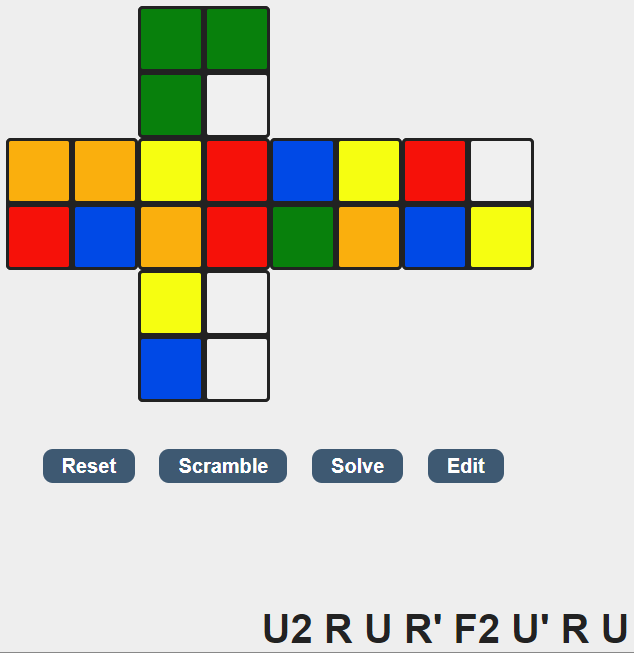
\includegraphics[width=7cm]{fig/case1}
  \quad
  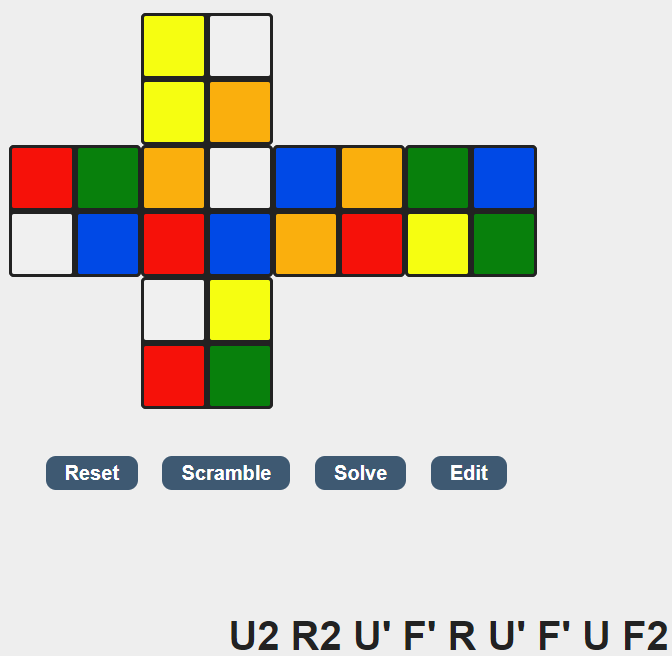
\includegraphics[width=7cm]{fig/case2}
  \caption{$2\times 2$ Rubik's Cube case1 and case2 }
\end{figure}
\begin{figure}[ht]
  \centering
  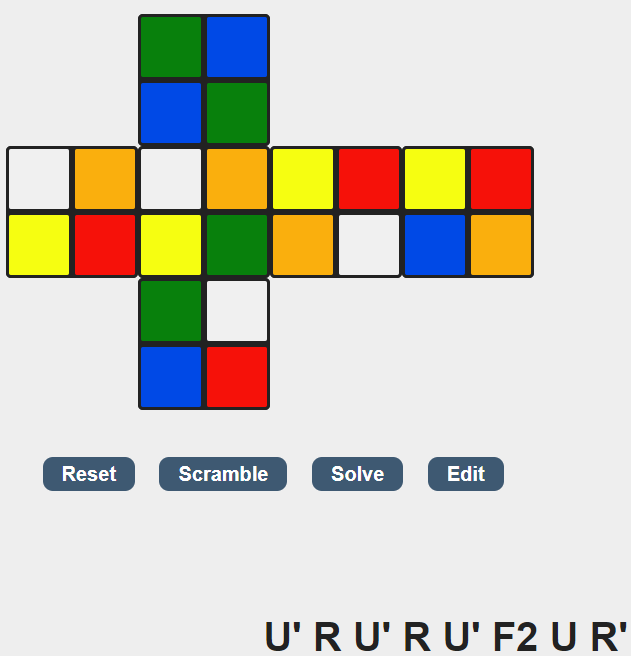
\includegraphics[width=7cm]{fig/case3}
  \quad
  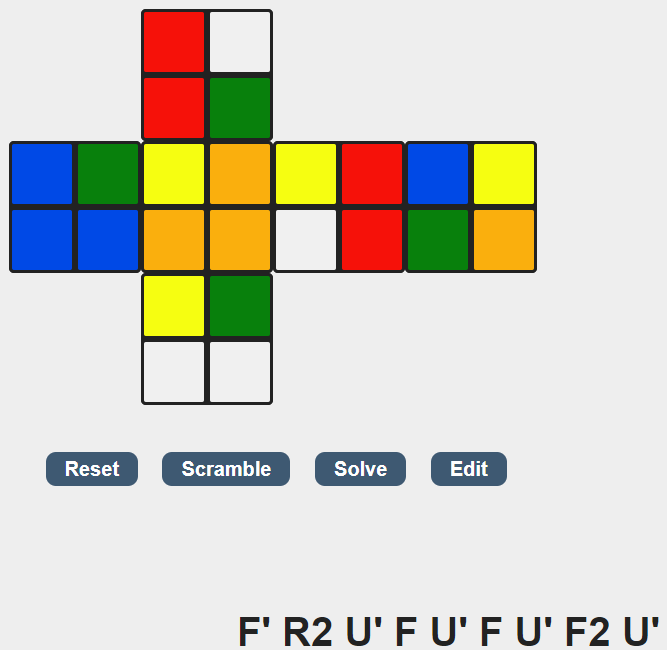
\includegraphics[width=7cm]{fig/case4}
  \caption{$2\times 2$ Rubik's Cube case3 and case4}
\end{figure}

\begin{figure}[ht]
  \centering
  
  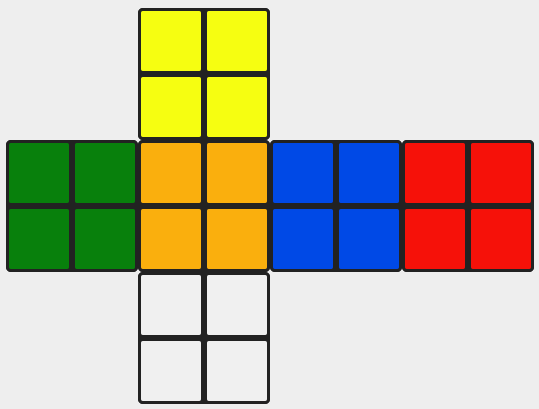
\includegraphics[width=8cm]{fig/goal}
  \caption{goal state}
\end{figure}

\newpage
\section{Diagnosing by Bayesian Networks}
\label{sec:bayesian-networks}
\textbf{2.1 Variables and their domais}
\begin{lstlisting}{language=Python}
(1)PatientAge:['0-30','31-65','65+']
(2)CTScanResult:['Ischemic Stroke','Hemmorraghic Stroke']
(3)MRIScanResult: ['Ischemic Stroke','Hemmorraghic Stroke']
(4)StrokeType: ['Ischemic Stroke','Hemmorraghic Stroke', 'Stroke Mimic']
(5)Anticoagulants: ['Used','Not used']
(6)Mortality:['True', 'False']
(7)Disability: ['Negligible', 'Moderate', 'Severe']
\end{lstlisting}
\textbf{2.2 CPTs}

\textbf{Note:} [CTScanResult, MRIScanResult,StrokeType] means:

P(StrokeType='...' $|$ CTScanResult='...' $\land$  MRIScanResult='...') 
\begin{lstlisting}{language=Python}
(1)
[PatientAge]

['0-30', 0.10],
['31-65', 0.30],
['65+', 0.60]

(2)
[CTScanResult]

['Ischemic Stroke',0.7],
[ 'Hemmorraghic Stroke',0.3]

(3)
[MRIScanResult]

['Ischemic Stroke',0.7],
[ 'Hemmorraghic Stroke',0.3]

(4)
[Anticoagulants]

[Used',0.5],
['Not used',0.5]

(5)
[CTScanResult, MRIScanResult,StrokeType])

['Ischemic Stroke','Ischemic Stroke','Ischemic Stroke',0.8],
['Ischemic Stroke','Hemmorraghic Stroke','Ischemic Stroke',0.5],  
[ 'Hemmorraghic Stroke','Ischemic Stroke','Ischemic Stroke',0.5],
[ 'Hemmorraghic Stroke','Hemmorraghic Stroke','Ischemic Stroke',0], 

['Ischemic Stroke','Ischemic Stroke','Hemmorraghic Stroke',0],
['Ischemic Stroke','Hemmorraghic Stroke','Hemmorraghic Stroke',0.4], 
[ 'Hemmorraghic Stroke','Ischemic Stroke','Hemmorraghic Stroke',0.4],
[ 'Hemmorraghic Stroke','Hemmorraghic Stroke','Hemmorraghic Stroke',0.9],

['Ischemic Stroke','Ischemic Stroke','Stroke Mimic',0.2],
['Ischemic Stroke','Hemmorraghic Stroke','Stroke Mimic',0.1],    
[ 'Hemmorraghic Stroke','Ischemic Stroke','Stroke Mimic',0.1],
[ 'Hemmorraghic Stroke','Hemmorraghic Stroke','Stroke Mimic',0.1],

(6) 
[StrokeType, Anticoagulants, Mortality]

['Ischemic Stroke', 'Used', 'False',0.28],
['Hemmorraghic Stroke', 'Used', 'False',0.99],
['Stroke Mimic', 'Used', 'False',0.1],
['Ischemic Stroke','Not used', 'False',0.56],
['Hemmorraghic Stroke', 'Not used', 'False',0.58],
['Stroke Mimic', 'Not used', 'False',0.05],

['Ischemic Stroke',  'Used' ,'True',0.72],
['Hemmorraghic Stroke', 'Used', 'True',0.01],
['Stroke Mimic', 'Used', 'True',0.9],
['Ischemic Stroke',  'Not used' ,'True',0.44],
['Hemmorraghic Stroke', 'Not used', 'True',0.42 ],
['Stroke Mimic', 'Not used', 'True',0.95]

(7)
[StrokeType, PatientAge, Disability]

['Ischemic Stroke',   '0-30','Negligible', 0.80],
['Hemmorraghic Stroke', '0-30','Negligible', 0.70],
['Stroke Mimic',        '0-30', 'Negligible',0.9],
['Ischemic Stroke',     '31-65','Negligible', 0.60],
['Hemmorraghic Stroke', '31-65','Negligible', 0.50],
['Stroke Mimic',        '31-65', 'Negligible',0.4],
['Ischemic Stroke',     '65+'  , 'Negligible',0.30],
['Hemmorraghic Stroke', '65+'  , 'Negligible',0.20],
['Stroke Mimic',        '65+'  , 'Negligible',0.1],

['Ischemic Stroke',     '0-30' ,'Moderate',0.1],
['Hemmorraghic Stroke', '0-30' ,'Moderate',0.2],
['Stroke Mimic',        '0-30' ,'Moderate',0.05],
['Ischemic Stroke',     '31-65','Moderate',0.3],
['Hemmorraghic Stroke', '31-65','Moderate',0.4],
['Stroke Mimic',        '31-65','Moderate',0.3],
['Ischemic Stroke',     '65+'  ,'Moderate',0.4],
['Hemmorraghic Stroke', '65+'  ,'Moderate',0.2],
['Stroke Mimic',        '65+'  ,'Moderate',0.1],

['Ischemic Stroke',     '0-30' ,'Severe',0.1],
['Hemmorraghic Stroke', '0-30' ,'Severe',0.1],
['Stroke Mimic',        '0-30' ,'Severe',0.05],
['Ischemic Stroke',     '31-65','Severe',0.1],
['Hemmorraghic Stroke', '31-65','Severe',0.1],
['Stroke Mimic',        '31-65','Severe',0.3],
['Ischemic Stroke',     '65+'  ,'Severe',0.3],
['Hemmorraghic Stroke', '65+'  ,'Severe',0.6],
['Stroke Mimic',        '65+'  ,'Severe',0.8]
\end{lstlisting}
\textbf{2.3 Calculation}

Please implement the VE algorithm (C++ or Python) to calculate the following probability value:

p1 = P(Mortality='True' $\land$ CTScanResult='Ischemic Stroke' $|$ PatientAge='31-65' )

p2 = P(Disability='Moderate' $\land$ CTScanResult='Hemmorraghic Stroke' $|$ PatientAge='65+' $\land$  MRIScanResult='Hemmorraghic Stroke')

p3 = P(StrokeType='Hemmorraghic Stroke' $|$ PatientAge='65+' $\land$ CTScanResult='Hemmorraghic Stroke' $\land$ MRIScanResult='Ischemic Stroke')

p4 = P(Anticoagulants='Used' $|$ PatientAge='31-65')

p5 = P(Disability='Negligible')


\section{Notes}

\begin{enumerate}
\item For task1, I will grade your codes in correctness of 4cases, the number of steps, and time cost.

\item For task2, I will grade your codes in VE implementation, correctness of 5 cases and algorithm efficiency.

\item Please send \textbf{P03\_YourNumber.zip} which should contain the codes and results of the above two problems to the mailbox (\textbf{ai\_201901@foxmail.com}) before the deadline (\textbf{2019/11/27 23:59}). 
\item Last but not least, you are not alone! If you find yourself stuck on something, contact the TA for help.
\end{enumerate}


\end{document}